\chapter{Spatial semantics}
\label{s:german-space-semantics}
So what is then the meaning of a phrase such as 
\textit{der Block links von der Kiste von dir aus} 
(`the block left of the box from your perspective')?
\figref{f:semantic-structure-der-block-links-der-kiste-von-dir-aus}
shows an IRL-network that agents autonomously construct to conceptualize
a particular spatial scene. The structure consists
of a set of cognitive operations that involve, for example, the construction of regions, 
the identification of landmarks, the application of perspective transformations and so on. But of course the network also contains references to spatial
categories, selectors, and other semantic entities that are processed by cognitive
operations. The following sections identify and describe the cognitive operations
and the semantic entities underlying locative utterances.

\begin{figure}
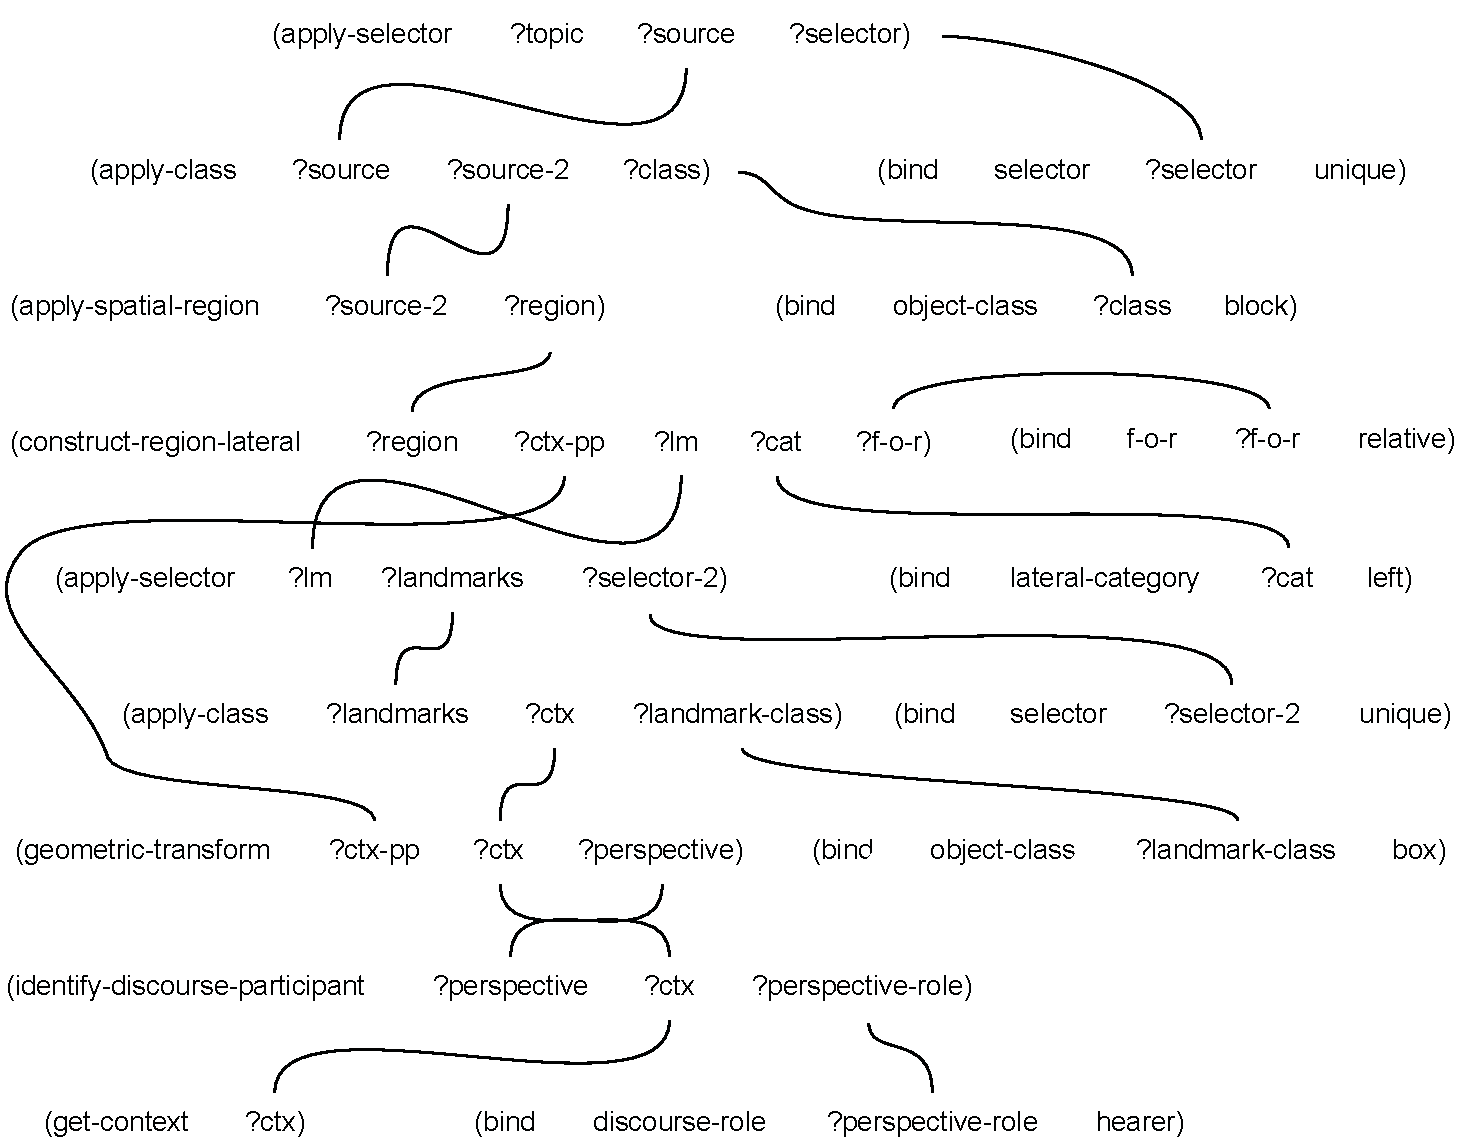
\includegraphics[width=\textwidth]{figs/semantic-structure-der-block-links-der-kiste-von-dir-aus}
\caption[Semantic structure of the phrase
\textit{der Block links von der Kiste von dir aus} 
(`the block left of the box from your perspective')]{%
An IRL-network representing the meaning of the phrase 
\textit{der Block links von der Kiste von dir aus} 
(`the block left of the box from your perspective')}
\label{f:semantic-structure-der-block-links-der-kiste-von-dir-aus}
\end{figure}

%%%%%%%%%%%%%%%%%%%%%%%%%%%%%%%%%%%%%
\section{Representing spatial relations}\is{spatial relation}
The semantics of spatial relations is the subject of ongoing debate. The 
key question is whether there is something like a 
\textsc{semantic core}\is{spatial relation!semantic core}  of 
spatial relations, i.e. a core meaning that 
abstracts from discourse situations as far as possible 
\citep{tenbrink2007space}\index{Tenbrink, T.}, and what that 
semantic core should be. For many scholars, the semantic core of spatial 
relations is related to geometric 
properties \citep{herskovits1986language,eschenbach1999geometric,tenbrink2007space}\index{Eschenbach, C.}\index{Herskovits, A.}\index{Tenbrink, T.}
in particular prototypical axis (directions) and distances defined using tools 
like lines, points, vectors, half-planes, etc. \citep{levinson1996language}\index{Levinson, S. C.}. 
Particularly, projective relations, e.g. \textit{vor} (`front') have been studied 
in this respect and certainly the class of absolute relations, e.g. \textit{n\"ordlich} 
(`north'), can be conceived in these terms. For instance, 
\cite{herskovits1986language}\index{Herskovits, A.}  describes the meaning 
of the spatial relation \textit{in front of} as graded concept with the frontal 
axis as the focal region. This conception links to another important property
of spatial language namely its inherent vagueness 
\citep{hall2008quantifying}\index{Hall, M. M.}\index{Jones, C. B.}.
Many of these proposals are rooted in a strand of psycholinguistic research that is concerned with
prototypes and prototypicality effects \citep{rosch1978principle}\index{Rosch, E.}. 
Here, prototypes or prototypical points in the sensorimotor
space are used as representations for spatial categories
(for a similar approach to color, see \citealt{bleys2010phd}\index{Bleys, J.}). 
For instance, the projective term \textit{links} (`left') can 
be interpreted for objects which relate to the reference object
by an angle of $90^\circ$ (prototypical left angle). The more the angle 
between the target object and the reference system deviates,
the less acceptable the spatial relation becomes \citep{tenbrink2005identifying,herskovits1986language,gapp1995angle}\index{Gapp, K.}\index{Tenbrink, T.}\index{Herskovits, A.}. 

In this section I focus on the geometric properties of spatial relations 
and combine them with the prototype approach to spatial categorization. 
There are two features of the sensorimotor space which are of particular
importance for spatial categorization: distance and angle. Two objects 
always have a certain distance from each other, and if there is a
coordinate system available which supports rotation also angles 
between objects can be measured. 
Consequently, from a computational point of view, there are two 
important category types for representing the geometric properties 
of the German spatial relations discussed in this book {\footnotesize\tt angular-category}, 
which represent prototypical angles and {\footnotesize\tt proximal-category}, 
which represent prototypical distances (see Figure \ref{f:category-hierarchy} for an overview).\is{spatial relation!proximal}

\begin{figure}
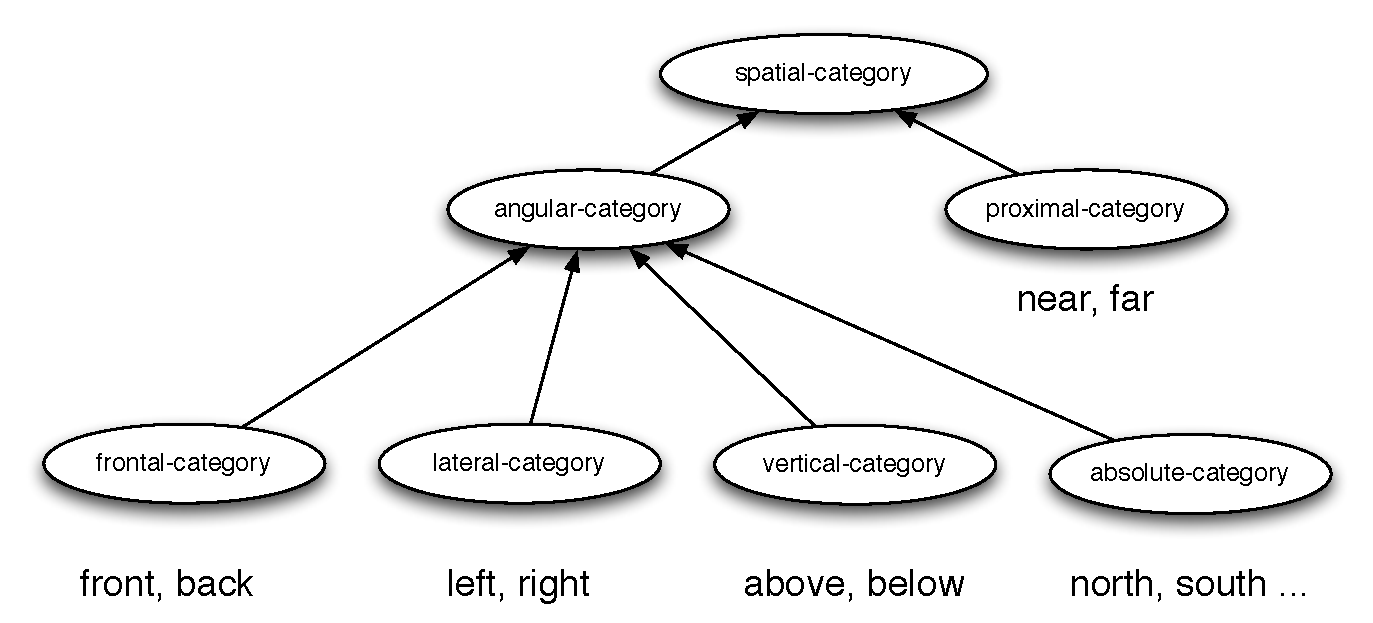
\includegraphics[width=1\columnwidth]{figs/category-hierarchy.pdf}
\caption[Category type hierarchy]{Category type hierarchy 
used in semantic processing}
\label{f:category-hierarchy}
\end{figure}

\subsection{Angular relations} 
The core semantics of spatial relations is represented
using functions that map a particular input location to the applicability degree 
of a particular category. For prototype based spatial categories 
degree of applicability amounts to similarity in some spatial dimension, 
e.g. in the angular dimension for angular relations. 
Projective and absolute relations are\is{spatial relation!projective}\is{spatial relation!absolute}\is{spatial relation!angular}
examples of angular categories, with a focal region around the 
denoted axis. For instance, frontal categories have a high degree of applicability
along the frontal axis. Whereas lateral categories have a high 
degree of applicability along the left and right axis. Similarly, 
absolute categories have high values of applicability
in their respective direction (see \figref{f:prototypical-spatial-relations} 
for an overview). In other words, for angular categories, 
similarity of some location to the category depends on the distance
of angles. In order to get a similarity function $\operatorname{sim}_{a} \in [0,1]$
the angle distance is wrapped in an exponential decay envelope 
and weighted by a $\sigma$ which steers the steepness of the 
exponential decay. High values for $\sigma$ correspond to a slow decay 
in similarity the bigger the angular distance, whereas low values for $\sigma$ 
correspond to a sharper decline in similarity.
Consequently, the following equations defines the degree of applicability given a
location $l$ and an angular category $c$, as the angular distance 
between $c$ and $l$, weighted by $\sigma$ and run through an exponential
decay.
\begin{eqnarray}
\label{e:angular-category-similarity}
\operatorname{sim}_{a}(l,c)&:=&e^{-\frac{1}{2 \sigma_c} d_a(l,c)}\\
\label{e:angular-distance}
d_a(l,c)&:=&|a_l - a_c|
\end{eqnarray}
In this definition $a_l$ denotes the angle of the position of location $l$ 
to the coordinate center and $a_c$ denotes the prototypical angle of the 
category $c$. Given this definition, one can go ahead and define 
angular categories, in particular I need to define the prototypical
angle for each angular category and the $\sigma$. 
Examples of definitions of angular spatial relations are 
depicted in \figref{f:prototypical-spatial-relations}. 


\subsection{Proximal relations} 
Proximal relations relate to some prototypical
distance. Two relations are modeled: {\footnotesize\tt near} and 
{\footnotesize\tt far}. The only difference to the definition of angular
categories is that proximal relations rely on the distance channel.
\begin{eqnarray}
\label{e:proximal-category-similarity}
\operatorname{sim}_{d}(l,c)&:=&e^{-\frac{1}{2 \sigma_c} d_d(l,c)}\\
\label{e:proximal-distance}
d_d(l,c)&:=&|d_l-d_c|
\end{eqnarray}
In this definition $d_l$ denotes the distance of the location $l$ 
to the coordinate center and $d_c$ denotes the prototypical 
distance of the category $c$.

\begin{figure}
\label{f:prototypical-spatial-relations}
\begin{center}
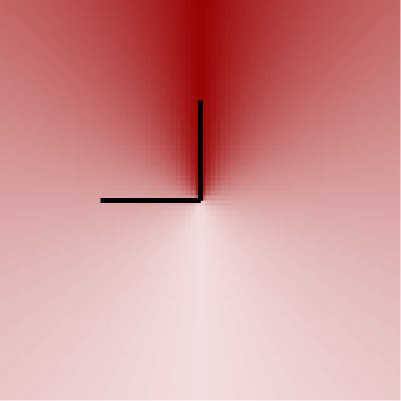
\includegraphics[width=0.15\columnwidth]{figs/categorization-front.jpg}

\includegraphics[width=0.15\columnwidth]{figs/categorization-back.jpg}
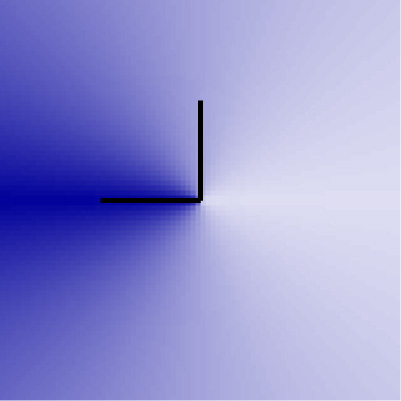
\includegraphics[width=0.15\columnwidth]{figs/categorization-left.jpg}

\includegraphics[width=0.15\columnwidth]{figs/categorization-right.jpg}
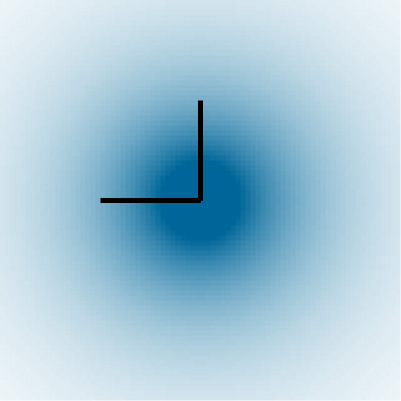
\includegraphics[width=0.15\columnwidth]{figs/categorization-near.jpg}

\includegraphics[width=0.15\columnwidth]{figs/categorization-far.jpg}
\end{center}
\caption[Degree of acceptability for projective and proximal categories.]{%
Degrees of acceptability shown for prototypical representation of frontal 
and lateral projective categories. From left to right {\footnotesize\tt front}, {\footnotesize\tt back},
 {\footnotesize\tt left}, {\footnotesize\tt right}, {\footnotesize\tt near} and {\footnotesize\tt far} are shown. 
 The opacity of each color denotes acceptability for a particular location in space ($x$-axes and $y$-axes 
 each run from $-2000.0$ to $2000.0$). 
 {\footnotesize\tt Front}, for instance, shows a strong acceptability along the $x$-axes. Definitions of 
categories are $a_{\mathtt{\footnotesize front}}=0.0$, $a_{\mathtt{\footnotesize back}}=\pi$, 
$a_{\mathtt{\footnotesize left}}=\frac{\pi}{2}$ and $a_\mathtt{{\footnotesize left}}=-\frac{\pi}{2}$ and
$\sigma_{\mathtt{\footnotesize front}}=\sigma_{\mathtt{\footnotesize\ back}}=\sigma_\mathtt{{\footnotesize left}}=\sigma_{\mathtt{\footnotesize right}} = 1.0$.
For absolute categories the same definitions exist with {\footnotesize\tt north} being defined like {\footnotesize\tt front}
and so forth.
The two proximal categories {\footnotesize\tt near} and {\footnotesize\tt far} are defined 
with $d_{\mathtt{\footnotesize near}}=0.0$, $a_{\mathtt{\footnotesize far}}=2000.0$ and 
$\sigma_{\mathtt{\footnotesize near}=700.0}$ and $\sigma_{\mathtt{\footnotesize far}}=1200.0$.}
\end{figure}


%%%%%%%%%%%%%%%%%%%%%%%%%%%%%%%%%%%%%
\section{Applying spatial relations}\is{spatial relation!regions}
Prepositionally and adverbially expressed spatial relations denote 
\textsc{spatial regions} which are always related to some reference object.
For instance, in the phrase \textit{der block links der Kiste} (`the block to the left
of the box') an object \textit{der Block} (`the block') is related to the landmark 
\textit{die Kiste} (`the box') via the spatial category \textit{links} (`left'). 
The information about which category is used and which landmark
is referred to is packaged in a spatial region.
In order to represent the difference between the construction of a region
as for instance denoted by the prepositional phrase \textit{vor der Kiste}
(`in front of the box') and the application of that region to filter objects,
as in the phrase \textit{der Block vor der Kiste} (`the block in front of the region'),
in other words in order to represent spatial relations, spatial 
processing is split into two distinct semantic operations. One operation
constructs the region and packages the particular landmark and the particular
spatial category, the other applies the region as a spatial relation 
to the objects available in the context.

\subsection{Spatial regions and spatial relations}
Proximal regions are computed based on the distance prototype of the 
corresponding category and the landmark. The semantic operation
{\footnotesize\tt construct-region-proximal} therefore constructs a specific 
region based on a spatial category and a landmark. 
The right image in \figref{f:apply-proximal-region} 
shows an example of a proximal region. 

\definition{Semantic operation}{construct-region-proximal}
\begin{explanation}{description}
Computes a proximal region based on the landmark.
\end{explanation}
\begin{explanation}{arguments}
{\footnotesize\verb+?spatial-region+} (of type spatial-region) \\
{\footnotesize\verb+?source-set+} (of type entity-set) \\
{\footnotesize\verb+?landmark+} (of type point)\\
{\footnotesize\verb+?category+} (of type proximal-category)
\vspace{0.3cm}
\end{explanation}

The other operation needed for applying a region is called 
{\footnotesize\tt apply-spatial-region}. This operation computes the similarity of 
every object in the context, given a region constructed, for instance by the 
operation {\footnotesize\tt construct-proximal-region}. For the case of 
a proximal region, this involves (1) transforming the context so
that the landmark is at the center of origin of the coordinate system
and (2) applying the similarity function defined in Equation 
\ref{e:proximal-category-similarity}. This operation in many ways
acts as a classifier such as the semantic operations for {\footnotesize\tt color}
and {\footnotesize\tt object-class} described in \chapref{s:irl}. 
For each object in the source set the similarity of this object to the 
spatial region is computed, based on the constituents of the region,
e.g. which category and which landmark was used to define the region.
This similarity is combined with the other computed similarities for
the object (see \chapref{s:irl} for description). 
The operation {\footnotesize\tt apply-region-filter} 
is general enough to be applicable to all regions, including projective and absolute 
regions whose description is to follow.\footnote{This operation can
be very general because its implementation defers different
methods of computing similarity for different category types
using the method dispatching facility of lisp.}

\definition{Semantic operation}{apply-spatial-region}
\begin{explanation}{description}
Applies a spatial region, by computing the similarity of the region
with every entity in {\footnotesize\verb+?source-set+}.
\end{explanation}
\begin{explanation}{arguments}
{\footnotesize\verb+?target-set+} (of type entity-set) \\
{\footnotesize\verb+?source-set+} (of type entity-set) \\
{\footnotesize\verb+?region+} (of type spatial-region)
\vspace{0.3cm}
\end{explanation}

An example of the interplay of the operations 
{\footnotesize\tt construct-region-proximal} 
and {\footnotesize\tt apply-region-filter} for
a spatial scene can be seen in
\figref{f:apply-proximal-region}. The following table 
summarizes the similarities computed when applying 
the region to the context (\figref{f:apply-proximal-region}
left).

\begin{center}
\begin{tabular}{lSS}
\lsptoprule
object & \multicolumn{1}{l}{distance (mm)} & \multicolumn{1}{l}{similarity} \\
\midrule
robot-1 & 1041.02 & 0.48 \\
robot-2 & 1224.53 & 0.42 \\
box-1 & 0.00 & 0.00\\
obj-266 & 419.97 & 0.74\\
obj-265 & 938.99 & 0.51 \\
\lspbottomrule
\end{tabular}
\end{center}


\begin{figure}
\begin{centering}
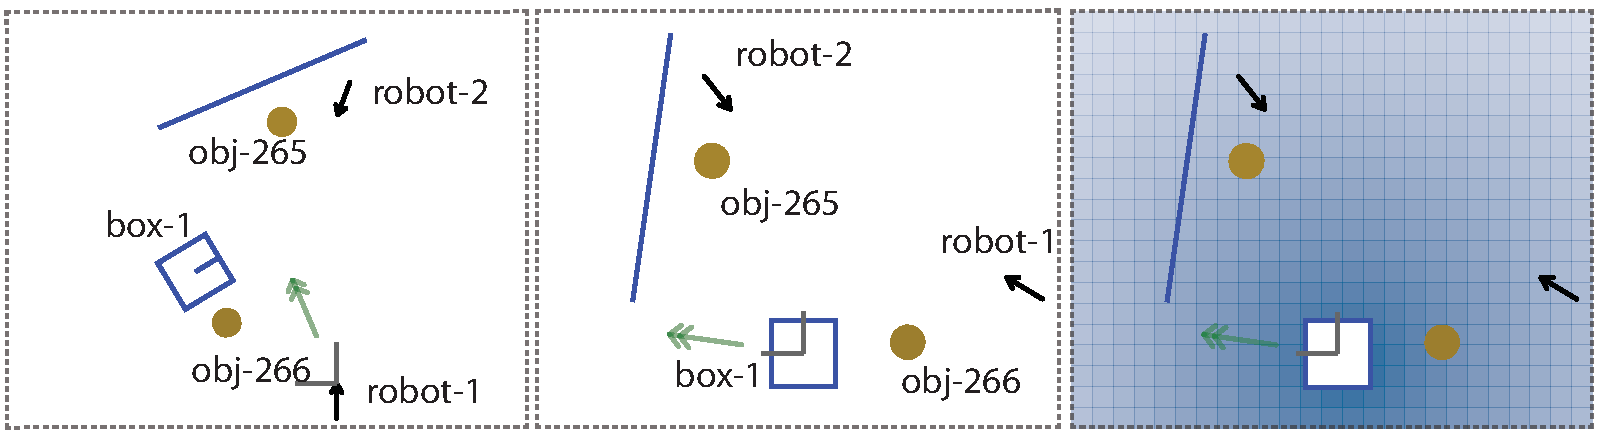
\includegraphics[width=\textwidth]{figs/space-scene-3-speaker-apply-proximal-region.pdf}
\end{centering}
\caption[Steps involved in applying a spatial relations.]
{When a region is applied, first, the context (left figure) is transformed so that
the landmark is at the origin of the coordinate system (middle figure) which is followed by the 
application of the spatial relation (right figure). Here, these steps are 
depicted for the category {\footnotesize\tt near} and the landmark {\footnotesize\tt box-1}.}
\label{f:apply-proximal-region}
\end{figure}

\section{Frames of reference}\is{frames of reference}
Projective and absolute relations are defined in terms of focal directions.
Consequently, for these kinds of relations the rotation of the landmark 
is an important issue determining the precise applicability of 
these relationships. For example, what is considered the front direction 
of a landmark has a direct effect on what is considered a frontal region. It turns out
that there is considerable amount of choice when it comes to how to
define the rotation of the landmark. The combination 
of a coordinate system, in particular its rotation, with a landmark is 
called \textsc{reference system}. Reference systems 
have been dealt with in great detail in cognitive semantics and 
psycholinguistics under the term \textsc{frame of reference}. 
\cite{levinson1996language,levinson2003space}\index{Levinson, S. C.} identifies 
three possible frames of reference: \textsc{intrinsic}, \textsc{relative} 
and \textsc{absolute}, all of which denote a particular way of construing 
a landmark for spatial relationships involving direction. 
In German all three frames of reference are possible.


\begin{description}
\item[Intrinsic frame of reference]\is{frames of reference!intrinsic}
The intrinsic frame of reference is an object centered coordinate 
system, meaning that projective categories are applied to the 
reference object based on particular sides of the object, which 
are construed as front, back, left and right. Hence, those objects 
that have something that can be considered as their front 
(with other sides, identifiable as well, e.g., left, right and back) 
are eligible to be used as landmarks with an intrinsic frame of 
reference. Examples of such objects are television sets, where 
the front is the screen, or houses, where the front is the main 
entrance or street access, and so forth.
\item[Relative frame of reference]
The relative frame of reference is a perspective based coordinate 
system. (See \figref{f:frames-of-reference} for a graphical 
explanation.) Instead of relying on intrinsic features of the 
reference object for determining the particular layout of the 
coordinate system, the rotation of the coordinate system is 
determined by its angle to an explicitly or implicitly given 
perspective. Hence, the front of an object is induced by the 
particular perspective on the scene. For example, \textit{vor dem 
Baum} (`in front of the tree') implicitly refers to a perspective, 
because trees do not have an intrinsically determined front, and 
it is the position of the observer together with the position of the 
tree that designates the precise region denoted as front.
\item[Absolute frame of reference] Absolute frames of reference construe 
the landmark using an external rotation. Neither intrinsic 
properties nor the perspective on the landmark determine the layout 
of the coordinate system, but rather geocentric features of the 
environment, for instance cardinal directions as in 
\textit{n\"ordlich} (`north') or the direction of gravity as in \textit{\"uber} (`above')
govern what the precise layout of the reference system is.
\end{description} 

\begin{figure}
\begin{center}
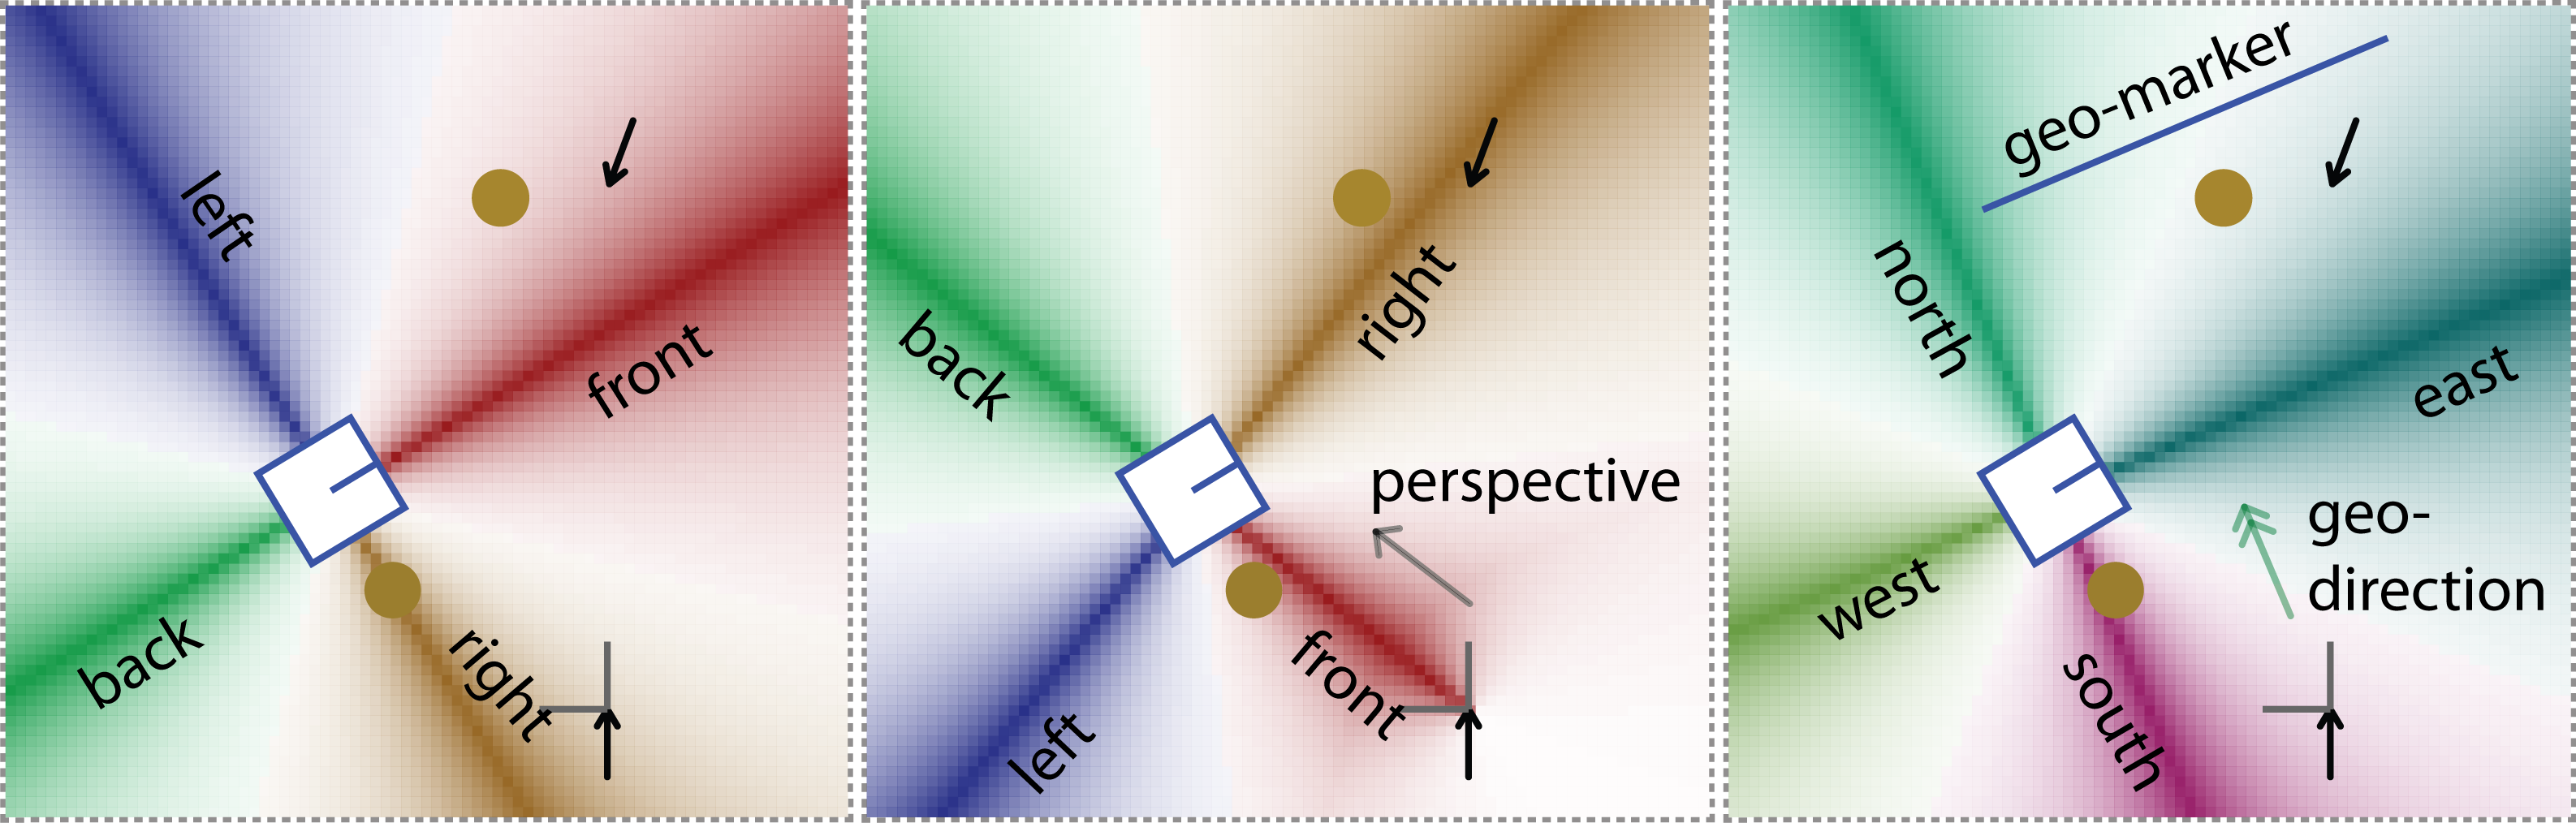
\includegraphics[width=1\columnwidth]{figs/space-scene-3-frames-of-reference.png}
\end{center}
\caption[Spatial relations and frames of reference.]
{Frames of reference have a profound effect on spatial relations. In all three
pictures spatial relations are shown with {\footnotesize\tt box-1} as reference object. The left
figure shows the landmark construed with an intrinsic frame of reference which
orients the coordinate system such that the front of the landmark 
(little blue line in the landmark) corresponds to the frontal spatial relation with
left, right and back projective relations aligned accordingly. The middle figure
shows the same landmark, but with a relative frame of reference constructed
from the perspective of robot {\footnotesize\tt robot-1} which entails that frontness 
corresponds to a region between the perspective and the landmark. 
Left and right in relative frames of reference are aligned not with respect to
front, but rather are parallel to the left and right side of the perspective 
{\footnotesize\tt robot-1}.
The right figure shows an absolute frame of reference applied to the landmark 
{\footnotesize\tt box-1}. Cardinal directions are aligned based on a geocentric direction
induced on the scene by a marker.\is{frames of reference!relative}}
\label{f:frames-of-reference}
\end{figure}


The differences in processing frames of reference are captured using 
distinct semantic operations. In other words, absolute relationships, 
such as \textit{n\"ordlich} (`north') or \textit{\"uber}  (`above') demand other semantic 
operations as relative and intrinsic ones. For instance, 
processing of phrases involving absolute regions, e.g. \textit{n\"ordlich}
(`north'), is represented using the {\footnotesize\tt construct-region-absolute} operation, 
which takes a landmark and transforms the context with respect to the 
landmark, subsequently applying a rotation that follows from a geocentric direction. 
Some of the spatial scenes recorded by the robots feature
a geocentric marker on the wall. The direction towards this marker
defines the direction to the north. Figure \ref{f:frames-of-reference} 
gives an example.

\is{frames of reference!absolute}
\definition{Semantic operation}{construct-region-absolute}
\begin{explanation}{description}
Computes an absolute region based on the landmark
and the absolute frame of reference which must be available
in source set.
\end{explanation}
\begin{explanation}{arguments}
{\footnotesize\verb+?spatial-region+} (of type spatial-region) \\
{\footnotesize\verb+?source-set+} (of type entity-set) \\
{\footnotesize\verb+?landmark+} (of type point)\\
{\footnotesize\verb+?category+} (of type absolute-category)
\vspace{0.3cm}
\end{explanation}

Frontal prepositions, e.g., \textit{vor} (`front') and \textit{hinter} (`back'), can have
both intrinsic and relative readings. Both readings are incorporated
into a single operation, which construes the landmark both
in relative and intrinsic way signified by an additional parameter
of type {\footnotesize\tt f-o-r} (frame of reference) to the operation.
For the relative reading the perspective on the scene additionally
influences the layout of the region. The viewpoint on
the scene constrains front regions in such a way that
only those locations which are between the perspective and
the landmark have a high degree of applicability.

\definition{Semantic operation}{construct-region-frontal}
\begin{explanation}{description}
Computes a frontal region based on the landmark
and the relative or intrinsic frame of reference.
\end{explanation}
\begin{explanation}{arguments}
{\footnotesize\verb+?spatial-region+} (of type spatial-region) \\
{\footnotesize\verb+?source-set+} (of type entity-set) \\
{\footnotesize\verb+?landmark+} (of type point)\\
{\footnotesize\verb+?f-o-r+} (of type f-o-r)\\
{\footnotesize\verb+?category+} (of type frontal-category)
\vspace{0.3cm}
\end{explanation}

Vertical relations can be construed with an absolute, relative
or intrinsic frame of reference. In the case of absolute frames
of reference the orientation is derived from gravity. For the purpose
of this book only absolute frames of reference readings are
implemented in the operation {\footnotesize\tt construct-region-vertical}.


%%%%%%%%%%%%%%%%%%%%%%%%%%%%%%%%%%%%%
\section{Internal and external regions}\is{spatial relation!internal}\is{spatial relation!external}
Another line of processing distinctions can be made between internal 
and external relations. \textit{North} and \textit{south}, but also prepositional use
of \textit{front}, e.g. \textit{vor}, are referring to external regions, that is the
region lies outside of the landmark. Internal regions on the other
hand lie inside the reference object. Adverbs such as \textit{vorne} (`front')
denote such regions inside the landmark. Consequently, they require
separate treatment and there is a specific operation
for handling the internal processing of frontal relations 
{\footnotesize\tt construct-region-frontal-internal}.

\definition{Semantic operation}{construct-region-frontal-internal}
\begin{explanation}{description}
Computes an internal frontal region based on the landmark
and the relative or intrinsic frame of reference.
\end{explanation}
\begin{explanation}{arguments}
{\footnotesize\verb+?spatial-region+} (of type spatial-region) \\
{\footnotesize\verb+?source-set+} (of type entity-set) \\
{\footnotesize\verb+?landmark+} (of type point)\\
{\footnotesize\verb+?f-o-r+} (of type f-o-r)\\
{\footnotesize\verb+?category+} (of type frontal-category)
\vspace{0.3cm}
\end{explanation}

Internal lateral regions are not clearly marked in syntax. 
While lateral prepositions clearly denote an external region, 
lateral adverbs can be used more varied which becomes apparent
since they can be complemented both by \textit{von} headed prepositonal
phrases, as well as \textit{in} headed prepositional phrases.
In other words, the interpretation of an adverb depends
on the complement. If there is no complement both readings
internal and external are possible. 

\definition{Semantic operation}{construct-region-lateral}
\begin{explanation}{description}
Computes an internal frontal region based on the landmark
and the relative or intrinsic frame of reference.
\end{explanation}
\begin{explanation}{arguments}
{\footnotesize\verb+?spatial-region+} (of type spatial-region) \\
{\footnotesize\verb+?source-set+} (of type entity-set) \\
{\footnotesize\verb+?landmark+} (of type point)\\
{\footnotesize\verb+?f-o-r+} (of type f-o-r)\\
{\footnotesize\verb+?category+} (of type frontal-category)\\
{\footnotesize\verb+?region-layout+} (of type region-layout)
\vspace{0.3cm}
\end{explanation}

%%%%%%%%%%%%%%%%%%%%%%%%%%%%%%%%%%%%
\begin{figure}
\begin{centering}
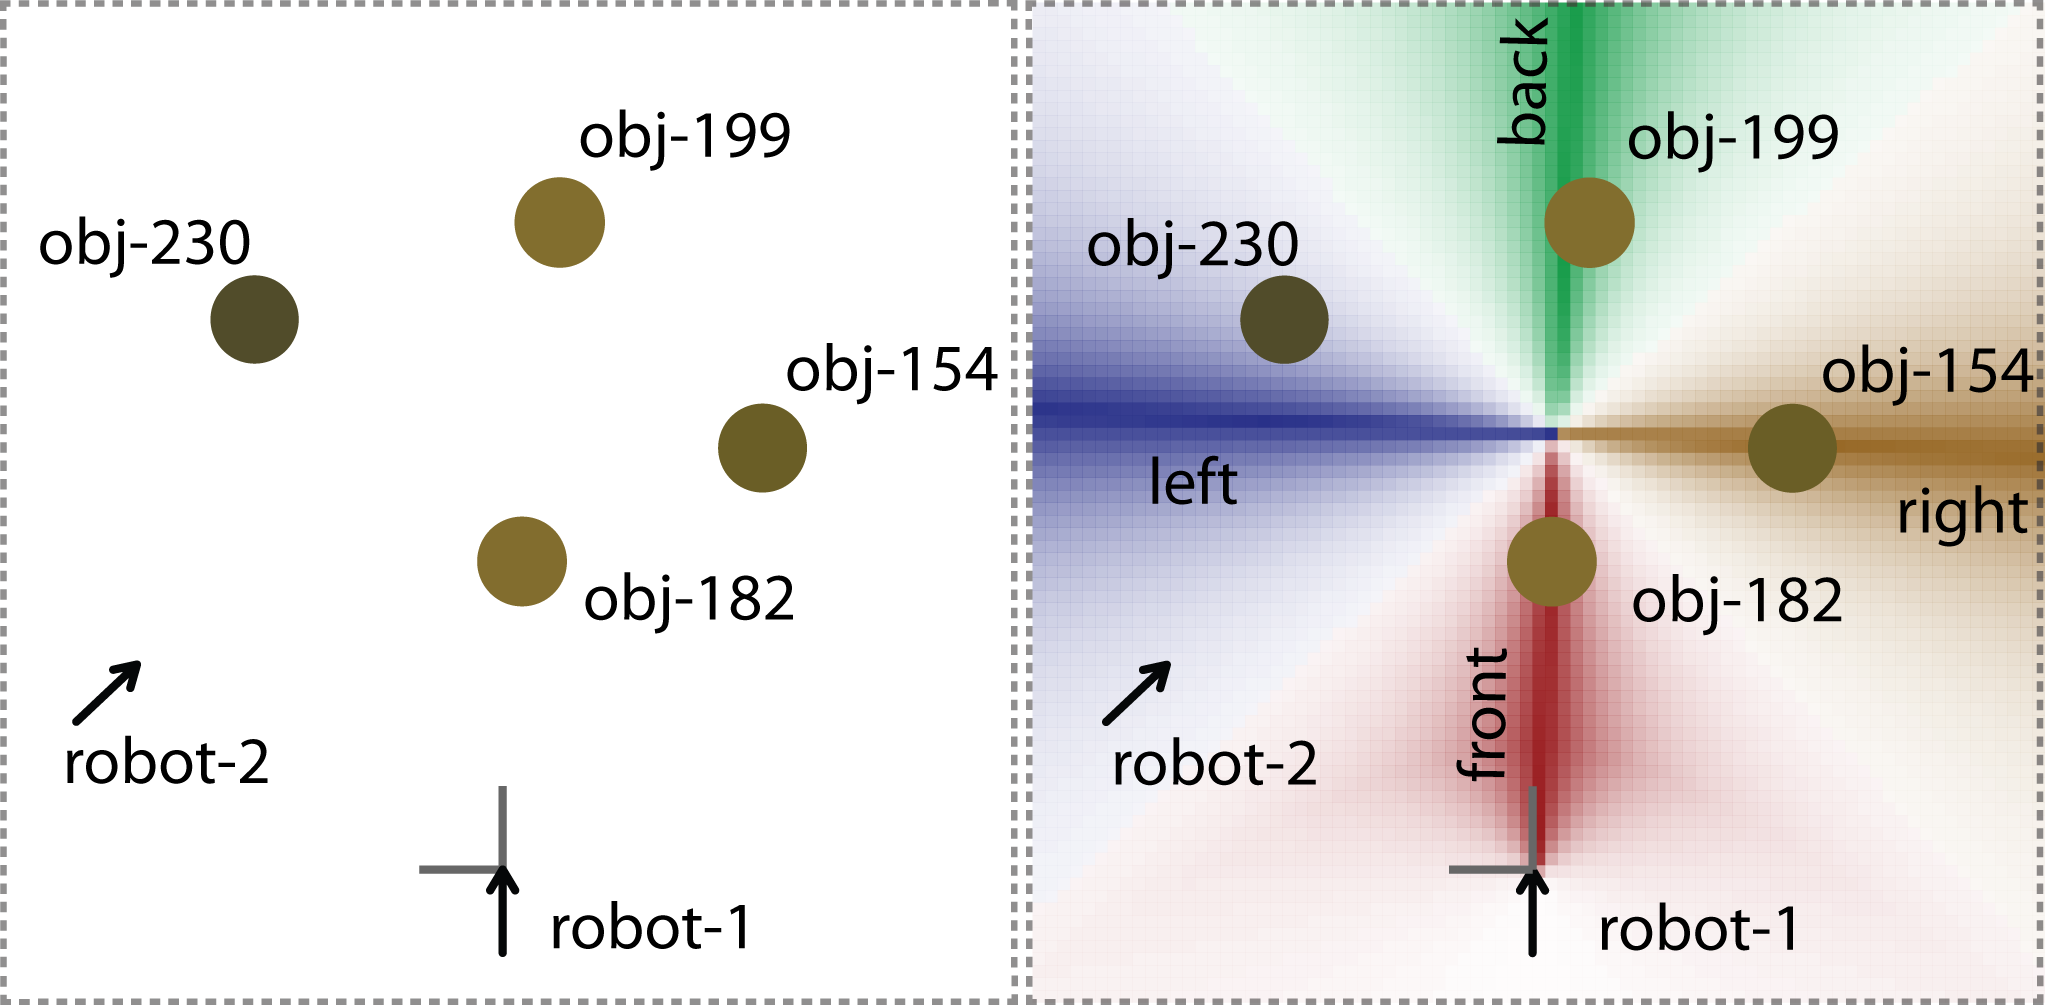
\includegraphics[width=0.7\columnwidth]{figs/space-scene-3483324847-group-based-reference.png}
\caption[Group-based reference explanation.]
{Group-based reference requires computing a landmark based on 
a group of objects. The centroid of the group of objects, in this case 
all blocks in the context, is construed using a relative frame of reference.
Consequently, object {\footnotesize\tt obj-182} could be described in German as 
\textit{der vordere Block} (`the front block').}
\label{f:6:space-scene-2}
\end{centering}
\end{figure}

\section{Group-based reference}\is{spatial relation!group-based reference}
The semantics of German spatial adjectives is best understood in terms of 
group-based reference.\footnote{Recent evidence \citep{moratz2006spatial}\index{Moratz, R.}\index{Tenbrink, T.} 
points to more variety in interpretation. For the purpose of this book, however,
I choose to model group-based semantics only.} In order for a group of objects 
to function as a reference object, the group needs to be construed as a landmark object, and in
particular its position needs to be established. One way of computing a position
for a group of objects, is to use the spatial centroid (center of mass) of the group 
as the position of the reference object. Additionally, a frame of reference, in other words
a rotation, needs to be chosen. This choice depends on the spatial relation. For
absolute relations the frame of reference is determined by an absolute 
frame of reference. In the absence of intrinsic features of the group of objects,
a relative frame of reference seems to be the natural choice, as a spatial group
of objects has no intrinsic front without including further constraints. 
Together, the centroid and the respective frame of reference sufficiently 
describe the reference system in order for spatial 
relations to be applied.

\definition{Semantic operation}{apply-spatial-category-group-based}
\begin{explanation}{description}
Applies the spatial category based on a group-based landmark. 
\end{explanation}
\begin{explanation}{arguments}
{\footnotesize\verb+?target-set+} (of type entity-set) \\
{\footnotesize\verb+?source-set+} (of type entity-set) \\
{\footnotesize\verb+?category+} (of type spatial-category)
\vspace{0.3cm}
\end{explanation}

Group-based reference offers a technical challenge of how to 
compute the group used for reference in the first place. Given that
all objects in the context are scored by successive operations, how can
a group of objects be established, in order to compute the
spatial centroid? For instance, in phrases like \textit{der linke block} (`the left block'),
the spatial adjective is part of a noun phrase, which primarily denotes the type of
objects that constitute a set, namely the set of all block which relates to 
the group that the reference should be based on.
The implementation of the semantic operation 
{\footnotesize\tt apply-spatial-category-group-based} relies on a well-known clustering algorithm
called $k$-means)\is{k-means@$k$-means} \citep{lloyd1982least}\index{Lloyd, S.P.} in order to find the group 
of objects in the input set. The scores of all objects in the input set 
are used to divide the input set into two groups and all elements 
in the group with the higher score centroid are used to compute 
the spatial landmark. 

%%%%%%%%%%%%%%%%%%%%%%%%%%%%%%%%%%%%%
\section{Perspective marking}\is{perspective marking}

\begin{figure}
\begin{center}
% LARGE_PDF
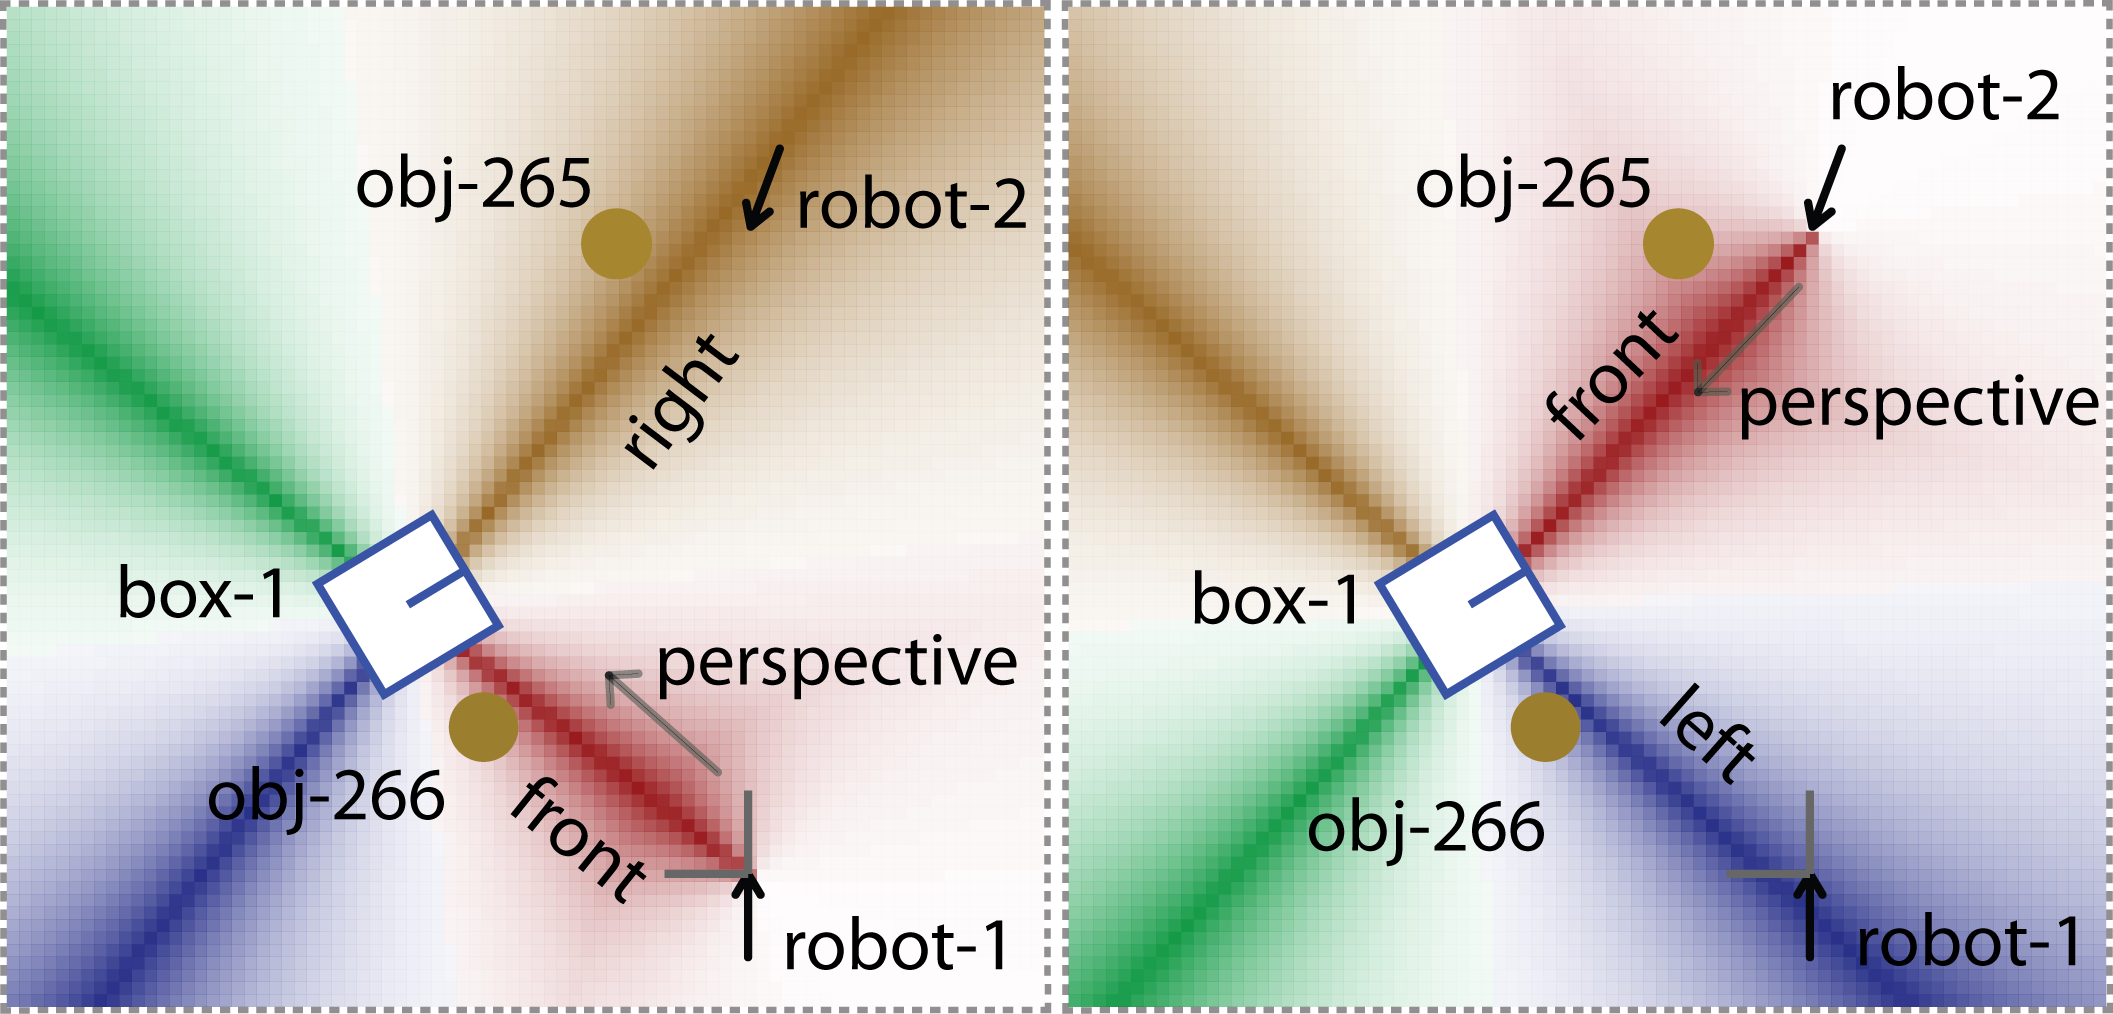
\includegraphics[width=0.7\columnwidth]{figs/space-scene-3-influence-perspective.png}
\caption[Influence of perspective on relative frames of reference.]
{The two figures show the influence perspective has on relative frames of reference.
The left figure shows the landmark {\footnotesize\tt box-1} when construed with a relative frame of reference
from the perspective of {\footnotesize\tt robot-1}. 
In this configuration object {\footnotesize\tt obj-266} is in front and object {\footnotesize\tt obj-265} is to the right.
Whereas when the same landmark {\footnotesize\tt box-1} is construed with a relative frame of reference
from the perspective of {\footnotesize\tt robot-2} it is object {\footnotesize\tt obj-265} which is in front,
whereas object {\footnotesize\tt obj-266} is to the left.}
\label{f:influence-perspective}
\end{center}
\end{figure}

The perspective of relative frames of reference is sometimes explicitly marked
by speakers. In the example \textit{der Block links von der Kiste von dir aus} (`the block left of the box from your perspective'),
the speaker choose to provide a perspective \textit{von dir aus} (`from your
perspective'). Only relative interpretations of a spatial phrase can be perspective 
marked. The perspective itself marks the position of the viewpoint, and therefore 
also the view direction, i.e. rotation. 

Intrinsic frames of reference computationally behave very similar to perspec\-tive-marked 
relative frames. Some argue therefore, that an intrinsic reference system is in essence a 
conflated relative reference system that coincides with the perspective 
on the scene \citep{levinson1996language}\index{Levinson, S. C.}. 
Hence, intrinsic reference systems are never perspective marked, since they already 
include position and orientation. However, perspective marking is only compatible with relative 
frames of reference and excludes intrinsic the usage
of intrinsic or absolute frames of reference. 
On the other hand, relative reference systems always explicitly or implicitly mark 
perspective, since they cannot be conceived without since by definition relative 
reference systems always construe the world from a perspective (see
\figref{f:influence-perspective}).

Perspective on a scene is changed by an operation that transforms
a complete spatial context as if it had been perceived from a 
particular viewpoint.

\definition{Semantic operation}{geometric-transform}
\begin{explanation}{description}
Transforms the context to be viewed from a particular perspective.
Notice that perspectives require both a particular point of view
but also a rotation.
\end{explanation}
\begin{explanation}{arguments}
{\footnotesize\verb+?transformed-context+} (of type sensory-context) \\
{\footnotesize\verb+?context+} (of type sensory-context) \\
{\footnotesize\verb+?perspective+} (of type pose)
\vspace{0.3cm}
\end{explanation}

%%%%%%%%%%%%%%%%%%%%%%%%%%%%%%%%%%%%%
\section{Discussion}

\subsection{Functional constraints}\is{spatial relation!functional constraints}
Purely geometric accounts of spatial semantics have been criticized
on the basis of psycholinguistic studies that reveal for many spatial relations,
that additional functional constraints influence their applicability. 
Studies in particular for topological relations,
including \emph{in} and \emph{on}, but also for projective relations such as 
\emph{over} and \emph{under} \citep{coventry2001}\index{Richards, L.}\index{Prat-Sala, M.}\index{Coventry, K.} as well as 
\emph{in front} and
\emph{behind} \citep{carlson1996influence}\index{Carlson-Radvansky, L. A.}\index{Radvansky, G. A.}  have led to new
proposals \citep{coventry2005spatial}\index{Rajapakse, R.}\index{Bacon, A.}\index{Joyce, D.}\index{Newstead, S.}\index{Cangelosi, A.}\index{Richards, L.}\index{Coventry, K.} as to how to include functional
considerations into the semantics of spatial terms (see also 
\cite{coventry2004saying}\index{Garrod, S.}\index{Coventry, K.} for an overview). For instance, 
whether or not an umbrella is \emph{over} a person depends on 
the direction of rain which can come from different angles. 
I do not account for
functional constraints for two reasons: (1) because it requires detailed
functional models of objects which as of now are rarely available
in robots and (2) the current model theoretically can incorporate such models
once they become available. In order to acquire functional 
knowledge, such as that chairs 
are for sitting, tables are used to put things on and so forth, 
robots need to interact robustly and repeatedly with objects 
of this kind, in particular using complex 
interactions in which objects take on functional roles. Many of
these skills, e.g. basic actions such as sitting,
are contemporary research fields in robotics and still need to see 
significant progress before they are generally 
available. On the other hand, functional approaches to semantics
are typically committed to conceive the application of spatial
relations in terms of degree of applicability. In other words, 
functional models are essentially mappings of
locations and landmarks to some number representing the
degree in which some relation is deemed acceptable. This is 
precisely the basis of the semantics advocated in this chapter.
Semantic operations compute degrees of applicability. Consequently, 
once a functional model can be established in terms of similarity,
it can readily be incorporated into the current model by exchanging
semantic operations.

\subsection{Contextual factors}\is{spatial relation!contextual factors}
Besides functional constraints, contextual factors affect the
applicability of spatial terms. For instance, for proximal relations: 
\textsc{prototypical size} \citep{gapp1994basic}\index{Gapp, K.}, but also 
\textsc{object salience} \citep{regier2001grounding}\index{Regier, T.}\index{Carlson, L. A.}, and \textsc{object interference} 
\citep{kelleher2009dialog}\index{Costello, F. J.}\index{Kelleher, J. D.} seem to play a role.
Just to give an example, the prototypical size factor can explain
why the proximal region \textit{nahe des Geb\"audes}
(`near the building') is larger than that of \textit{nahe dem Apfel} (`near the apple') 
(example adapted from \citealt{gapp1994basic}\index{Gapp, K.}) by the difference in typical 
size of buildings and apples. 
Constraints such as the prototypical size, as well as the influence of
object salience, are easily integrated into the model, but just as 
for functional constraints do not affect the basic assumptions
of the model. The third constraint -- the object interference constraint --
refers to the interference by other objects that are for
instance closer than the related object. Such constraints are better treated 
under the problem of how to choose spatial relations which is inevitably
connected to the particular communicative goal. 
For instance, in a discrimination task other categories
might be more relevant for the task than in object location description tasks.
Such processes are dealt with in detail in \chapref{s:german-locative-phrases-semantic-processing}.


\subsection{Other modeling approaches}\is{spatial relation!spatial ontologies}\is{spatial relation!qualitative spatial reasoning}
Spatial semantics is an important and vibrant research area. 
Many different proposals are currently being made. Some suggest 
the use of formal ontology engineering \citep{bateman2007role,bateman2010situating,bateman2010ontology}\index{Ross, R.}\index{Farrar, S.}\index{Bateman, J. A.}\index{Hois, J.}\index{Tenbrink, T.}
as a tool for enhancing spatial language interpretation by artificial 
systems. Others suggest to use formal reasoning techniques
and representations \citep{freksa1991qualitative,cohn2001qualitative}\index{Hazarika, S. M.}\index{Freksa, C.}\index{Cohn, A. G.}.
The system presented in this book can benefit from these
extensive approaches in the sense that the detailed modeling 
of spatial representation and spatial reasoning could enhance
our modeling approach. On the other hand, in this book modeling 
serves the goal of establishing basic concepts, e.g. spatial relations,
so that we can later study their evolution. This is the
reason why more elaborate modeling approaches are avoided. Engineering
robust and extensive solutions for the processing of spatial
language is a valid goal in itself, but it is only one aspect of 
this book.

\subsection{Summary}
This chapter gave an account of the semantic core 
of German spatial relations in terms of geometric constraints,
frames of reference and perspective. Spatial relations have been
defined as graded categories, whose application is governed
by semantic operations. It remains to be shown (1) how 
conceptualizations of a scene given a concrete communicative
goal are achieved (a problem that can be summarized in how and 
which spatial relations should be chosen),  (2) how spatial
categorization fits into larger semantic structures for spatial
phrases such as \textit{der Block links von der Kiste} and (3)
how these semantics interact with language in production 
and parsing of spatial phrases.